\documentclass[12pt,english]{report}
\usepackage[utf8]{inputenc}
\usepackage[a4paper,bindingoffset=0.2in,%
            left=0.4in,right=1in,top=1in,bottom=1in,%
            footskip=.25in]{geometry}
\usepackage{amsmath}
\usepackage{amssymb}
\usepackage{graphicx}
\usepackage{hyperref}
\usepackage{listings}
\usepackage{color}
\usepackage{booktabs}
\usepackage{biblatex}
% \usepackage{fancyhdr}

% \definecolor{dkgreen}{rgb}{0,0.6,0}
% \definecolor{gray}{rgb}{0.5,0.5,0.5}
% \definecolor{mauve}{rgb}{0.58,0,0.82}

% \lstset{frame=tb,
%   language=Matlab,
%   aboveskip=3mm,
%   belowskip=3mm,
%   showstringspaces=false,
%   columns=flexible,
%   basicstyle={\small\ttfamily},
%   numbers=none,
%   numberstyle=\tiny\color{gray},
%   keywordstyle=\color{blue},
%   commentstyle=\color{dkgreen},
%   stringstyle=\color{mauve},
%   breaklines=true,
%   breakatwhitespace=true,
%   tabsize=3
% }

\addbibresource{references.bib}

\graphicspath{ {./img/} }

% \pagestyle{fancy}

\title{Sistem IoT pentru controlul accesului in clădire}
\date{2021\\ Noiembrie}
\author{Ionescu Alexandru Cristian}


\begin{document}

\maketitle

\chapter*{Abstract}
Salut aici vorbesc io ceva abstract despre lucrarea asta.

\tableofcontents

\chapter{Solutii existente}
Majoritatea sistemelor de tip interfon, chiar si cele nou instalate, sunt realizate cu terminale de telefonie fixa datorita simplitudinii modului de operare. In esenta este nevoie de 4 fire pentru a avea o linie de telecomunicatie bi-directionala.

\href{https://www.epanorama.net/documents/telecom/telephone_intercom.html}{Simple schema}

\begin{figure}[h!]
  \centering
  \fbox {
    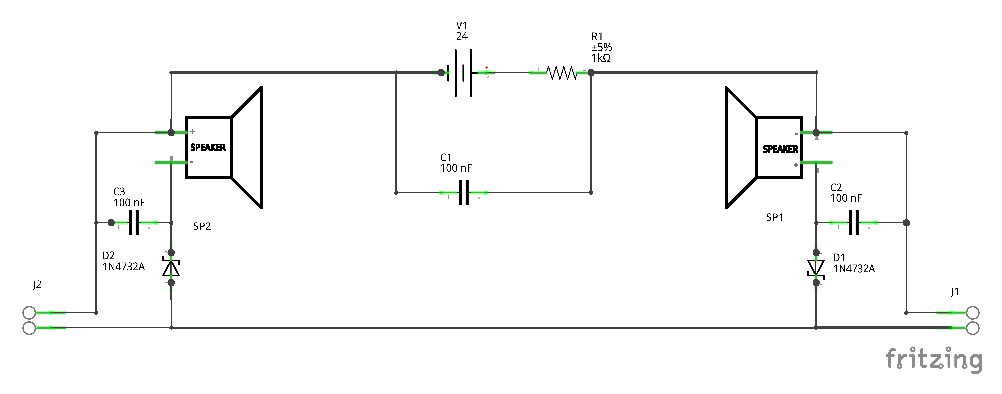
\includegraphics[width=0.8\textwidth]{01/interfon_schem.pdf}  
  }
  \caption{Schema simpla interfon cu speaker}
\end{figure}

\section {Plain Ordinary Telephone System}

Pentru a adauga mai multe terminale in retea, a fost dezvoltata tehnologia numita POTS (Plain Ordinary Telephone Service). Coordonarea acestui sistem este realizata de un decodor DTMF ce are rolul de a transforma semnalul modulat de pe linia X intr-o adresa din retea. 

\begin{figure}[h!]
  \centering
  \fbox {
    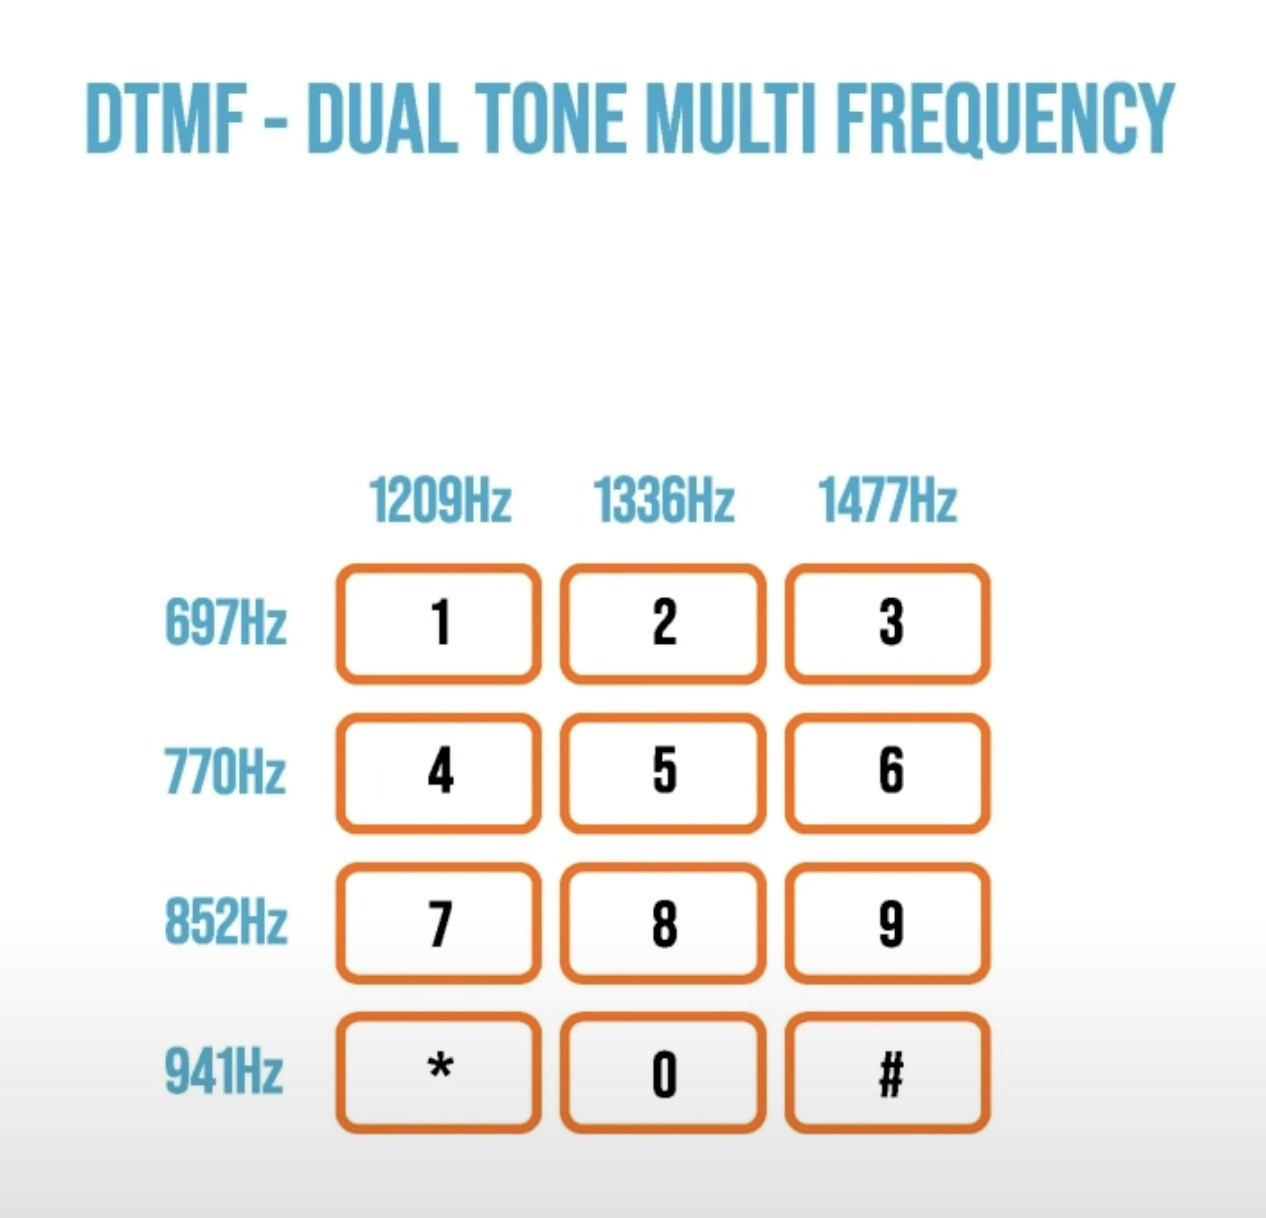
\includegraphics[width=0.8\textwidth]{01/dtmf.jpeg}  
  }
  \caption{Diagrama DTMF}
\end{figure}

In DTMF randurile sunt numite si GROUP JOS (cu frecvente intre 600 si 900 $Hz$), iar coloanele sunt numite GROUP INALT. Asadar, cand se apasa tasta 8 a unui terminal, frecventa de $852 Hz$ este aleasa din grupulul JOS si frecventa $1336 Hz$ sunt emise in acelasi timp.


Decodorul DTMF foloseste filtre Notch pentru acest procedeu.

\begin{figure}[h!]
  \centering
  \fbox {
    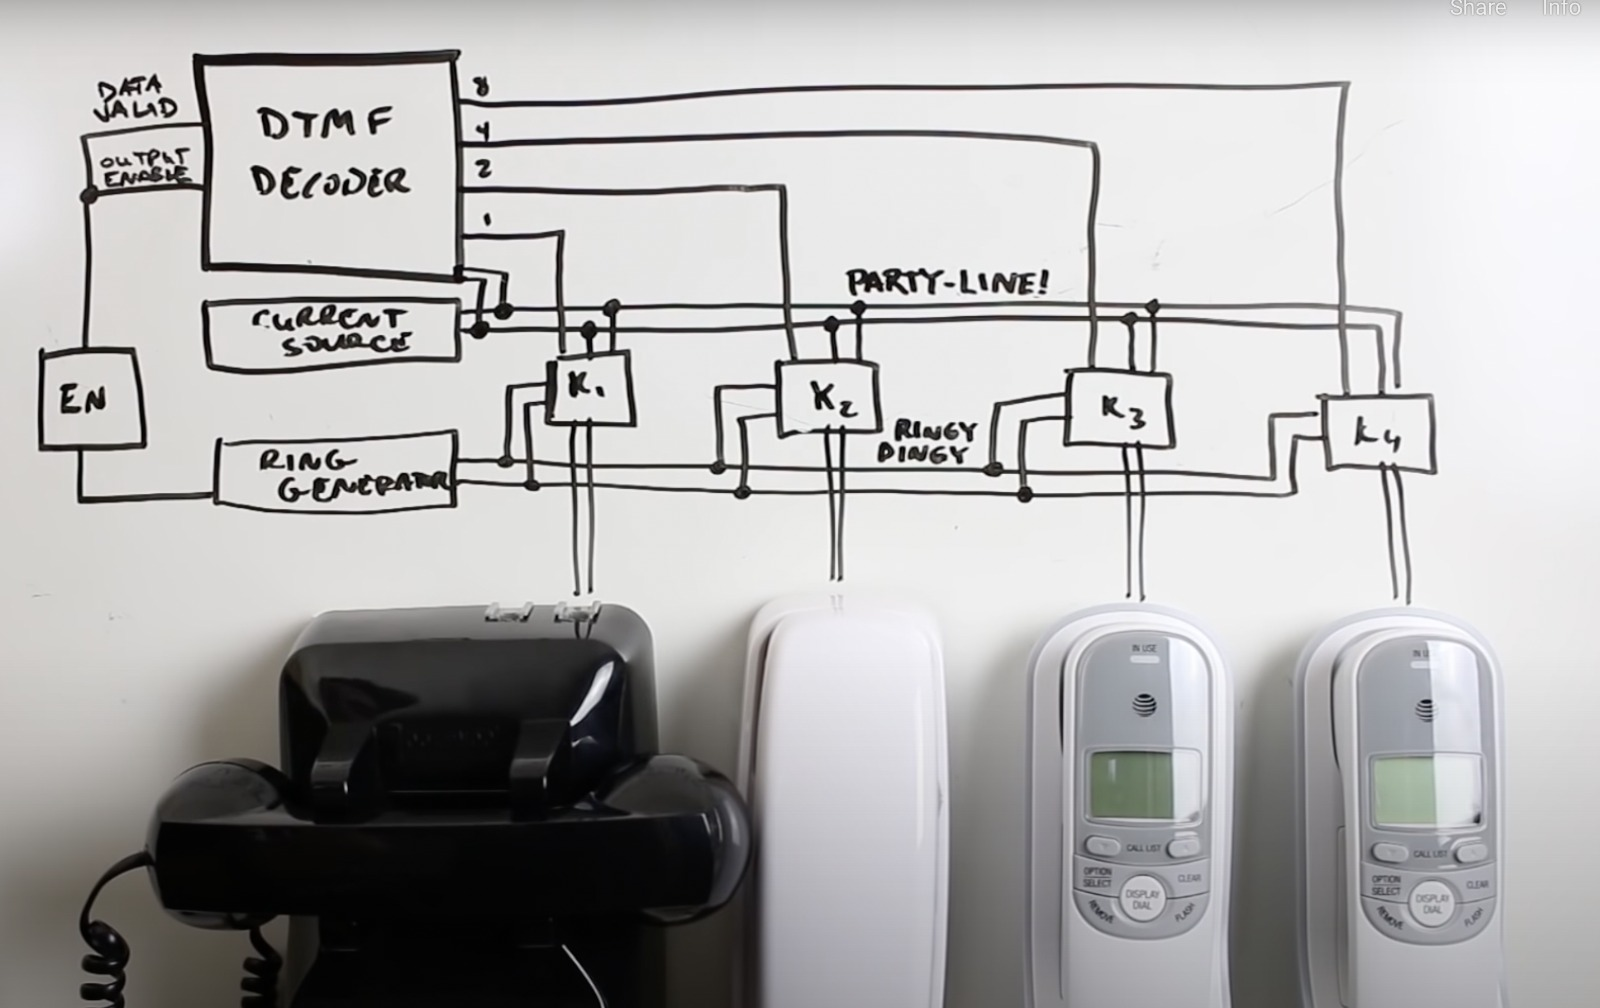
\includegraphics[width=0.8\textwidth]{01/schema_pots.jpeg}  
  }
  \caption{Schema sistem POTS}
\end{figure}

\cite{WinNT}



\href{https://www.nextiva.com/blog/what-is-pots.html}{Alt articol}

O evolutie normala de la acest sistem, ca si trecerea de la telefonul fix la cel mobil, sunt interfoanele GSM. Acestea dispun de un modul GSM cu o agenda ce are rolul de a oferi acces numerelor salvate sa interactioneze cu sistemul.


\section {Videx UK}

\href{https://www.videxuk.com/system/gsm-intercoms/}{Videx UK}


\section {Interfon GSM}

\href{https://www.a2t.ro/interfoane-videointerfoane/interfon-wireless-gsm-pentru-o-familie.html}{Link}

Interfon wireless GSM pentru o familie si controlere GSM pentru deschidere de porti sau bariere. Foarte util pentru zonele in care nu exista cablaje. Poate deschide o yala, o automatizare sau o bariera. Vorbesti cu vizitatorii direct de pe telefonul tau mobil. Functioneaza pe reteaua oricarui operator de telefonie mobila 2G.

\section {Hikvision DS-KV8413-WME1}

\href{https://www.a2t.ro/videointerfon-wireless/videointerfon-full-hd-4-familii-control-acces-aplicat-tcp-ip-hikvision-ds-kv8413-wme1-s.html}{Link}

\href{https://www.hikvision.com/content/dam/hikvision/products/S000000001/S000000083/S000000129/S000000131/OFR000170/M000048926/User_Manual/UD20207B_Baseline_Video-Intercom-8-Series-Villa-Door-Station_User-Manual_V2.2.3.PDF}{Manual}


Post de exterior, camera 2MP, WiFi Proxi, 4 butoane de apelare, reducere zgomot si ecou, audio bidirectional, BLC, DNR, WDR, IP65, IK08, PoE / 12VDC. Montaj ingropat.

Video-interfon metalic, cu 4 butoane (pentru 4 familii).


\chapter{Bill of Materials}
\section {Estimat}
\begin{minipage}{\textwidth}
  \centering
  \begin{tabular}{ lccc } 
    \midrule
    Part name & Quantity & Price & Provider \\
    \midrule
    \midrule
    Raspberry Pi Zero W & 1 & 58.05 RON & OptimusDigital\footnote{https://www.optimusdigital.ro/} \\

    Header de Pini Mamă 2x20p 2.54 mm & 1 & 3.99 RON & -\\ 

    Diodă 1N4007 & 4 & 1.96 RON & -\\ 

    Soclu de 14 pini & 1 & 0.99 RON & -\\ 

    Header de Pini Mamă 3p 2.54 mm & 1 & 0.49 RON & -\\ 

    LM324AN & 1 & 2 RON & Robofun\footnote{https://www.robofun.ro/generale/lm324an-amplificator-operational-dip14.html}\\ 

    IRF3205 & 1 & 3.99 RON & https://www.optimusdigital.ro/\\ 
    \midrule
  \end{tabular}
\end{minipage}




\printbibliography

\end{document}